%%%%%%%%%%%%%%%%%%%%%%%%%%%%%%%%%%%%%
% Note: This document can be build  %
% by using pdflatex and not latex   %
%%%%%%%%%%%%%%%%%%%%%%%%%%%%%%%%%%%%%
%
% Lade Dokumenttyp
% Die Kommentare zu diesem Befehl sind etwas länglich und stehen in latex/documentclass.tex
% Das sollte man sich mal durchlesen!
\documentclass[a4paper, 12pt, BCOR8.25mm, headsepline, final, bibliography=totoc, listof=totoc, index=totoc, parskip=half*, chapterprefix, appendixprefix, captions=nooneline, origlongtable]{scrbook}
%
% Lade Unterstützung für die deutsche Sprache
%
%%%%%%%%%%%%%%%%%%%
% Sprachcodierung %
%%%%%%%%%%%%%%%%%%%
\usepackage[T1]{fontenc}
% Paket fontenc: Fontencoding T1 festlegen, damit Wörter, die Umlaute
% enthalten richtig getrennt werden.
\usepackage[utf8]{inputenc}
% Paket inputenc: Unterstützung verschiedener Zeichenkodierungen.  Unterstützte
% Kodierungen sind:
% ascii		ASCII Kodierung für Zeichen in dem Bereich von 32 bis 127
% latin1	ISO Latin1
% latin2	ISO Latin2
% latin3	ISO Latin3
% latin4	ISO Latin4
% latin5	ISO Latin5
% latin9	ISO Latin9 (definiert die ISO 8859-15 Codierung einschließlich des EURO-Zeichnes: \texteuro)
% decmulti	DEC Multinational Character Set Encoding für das OpenVMS Betriebssystem
% cp437		IBM 437 Code Page
% cp437de	IBM 437 Code Page deutsche Version
% cp850		IBM 850 Code Page
% cp852		IBM 852 Code Page
% cp865		IBM 850 Code Page
% cp1250	Windows 1250 (Zentral- und Osteuropa) Code Page
% cp1252	Synonym für ansinew
% applemac	Macintosh Kodierung
% next		Next Kodierung
% ansinew	Windows 3.1 ANSI Kodierung, erweiterung von Latin1
% Dokumentation zu diesem Paket: /usr/share/doc/texmf/latex/base/inputenc.dvi.ps
%
\usepackage[english,ngerman]{babel}
% Paket babel: Unterstützung für andere Sprachen als amerikanisches Englisch
% Die Sprachen Englisch, Französich und Deutsch  verwenden. Die zuletzt aufgeführte
% Sprache ist die Sprache, die beim Start geladen wird. Zwischen den einzelnen
% Sprachen kann man mittels \selectlanguage{english}, \selectlanguage{ngerman} und
% \selectlanguage{french} umgeschaltet werden. ngerman steht für die neue, german
% für die alte deutsche Rechtschreibung.
% Mittels \iflanguage{sprache}{wahr-Klausel}{falsch-Klausel} kann abgeprüft werden,
% welche Sprache gerade aktiv ist und demensprechend können Befehle ausgeführt werden.
% Umlaute und Sonderzeichen mit dem babel Paket:
% ä = \"a 
% Ä = \"A
% ö = \"o 
% Ö = \"O
% ü = \"u 
% Ü = \"U
% ß = \"s
% SS = \"S ( groß geschriebene ß als SS wie z.B in STRASSE )
% Deutsche doppelte Anführungszeichen links unten \glqq
% Deutsche doppelte Anführungszeichen rechts oben \grqq
% Deutsche einfache Anführungszeichen links unten \glq
% Deutsche einfache Anführungszeichen rechts      \grq
% Französische doppelte Anführungszeichen links  \flqq
% Französische doppelte Anführungszeichen rechts \frqq
% Franz<F6>sische einfache Anf<FC>hrungszeichen links  \flq
% Franz<F6>sische einfache Anf<FC>hrungszeichen rechts \frq
% Original Anf<FC>hrungszeichen \dq
% Weitere Spezialbefehle zur Silbentrennung und Lignatur
% Dokumentation zu diesem Paket: /usr/share/doc/texmf/generic/babel/user.dvi.gz
\selectlanguage{ngerman}

%
% Lade persönliche Daten
% Dieses Dokument solltest Du auf jeden Fall anpassen, denn hier kommt Dein Name und der Titel Deiner Arbeit hinein.
% Hier werden Makros definiert, die in den folgenden LaTeX-Dokumenten verwendet werden.
%
%
% Die Art der Arbeit: Bachelorarbeit/Masterarbeit - einfach das richtige auskommentieren
% 
%\newcommand{\thethesis}[0]{Masterarbeit}
\newcommand{\thethesis}[0]{Bachelorarbeit}
%
% Der Titel Deiner Arbeit
%
\newcommand{\thesistitle}[0]{Meine Examensarbeit}
%
% Der Titel Deiner Arbeit in englisch
%
\newcommand{\thesistitleGB}[0]{My Master Thesis}
%
% Der formatierte Titel Deiner Arbeit für das erste Deckblatt
%
\newcommand{\thesisTitleFormatted}[0]{Meine\\Examensarbeit}
%
% Das Thema Deiner Arbeit (Kurzfassung des Titels)
%
\newcommand{\thesissubject}[0]{\thesistitle}
%
% Stichwörter, die Deine Arbeit charakterisieren
%
\newcommand{\thesiskeywords}[0]{DBMS; Datenbanksysteme; Datenbanken}
%
% Beginn Deiner Arbeit
%
\newcommand{\startofwork}[0]{01.12.2007}
%
% Abgabetag Deiner Arbeit
%
\newcommand{\dayofdoom}[0]{31.05.2008}
%
% Der Betreuer Deiner Arbeit
%
\newcommand{\tutor}{Dipl.-Inf.\ Florian Irmert}
%
% Dein Korrektor bzw. Professor
%
\newcommand{\corrector}[0]{Univ.-Prof.\ Dr.-Ing.\ habil.\ Klaus Meyer-Wegener}
%
% Dein Vor- und Nachname
%
\newcommand{\myname}[0]{Vorname Nachname}
%
% Dein Geburtstag
%
\newcommand{\birthday}[0]{01.01.2000}
%
% Dein Geburtsort
%
\newcommand{\birthplace}[0]{Erlangen}

%
% Lade Pakete
%
%%%%%%%%%%%%
% Tabellen %
%%%%%%%%%%%%
% Paket supertabular: Aufteilung von Tabellen auf mehrere Seiten bzw.
% Einbindung mehrseitige Tabellen. Die sind dann auch wirklich da, wo man sie vom Layout her hinsetzt :-)
\usepackage{multicol}
\usepackage{supertabular}
%
% Paket colortbl: Farbige Tabellenspalten
% Documentation:  CTAN:macros/latex/contrib/colortbl
\usepackage{colortbl}
%
% Paket booktabs: Trennlinien für Tabellen
\usepackage{booktabs}
%
%%%%%%%%%%%%%%%%%%%%%%%%%
% Programmcode Listings %
%%%%%%%%%%%%%%%%%%%%%%%%%
\usepackage{listings}
%
%%%%%%%%%
% Index %
%%%%%%%%%
% Paket makeidx: Zur Erstellung eines Index
\usepackage{makeidx}
% Erstellt einen Index
\makeindex
%
%%%%%%%%%%%%%%%%%%%%%%%%%%%%%%
% Bessere Bildunterschrfiten %
%%%%%%%%%%%%%%%%%%%%%%%%%%%%%%
\usepackage[justification=centerlast,format=hang,font=small,labelfont=bf]{caption}
%
%%%%%%%%%
% Farbe %
%%%%%%%%%
\usepackage{color}
%
%%%%%%%%%%%%
% Grafiken %
%%%%%%%%%%%%
% PDF als Grafiken einbinden
% Intern lädt dieses Paket das Paket graphicx automatisch.
%\usepackage[final]{pdfpages}
% Grafiken einbinden
\usepackage{graphicx}
% LaTeX-Inline-Grafiken
\usepackage{tikz}
\usetikzlibrary{shapes.multipart,shapes.symbols,positioning,calc,arrows}
% Mehrere Grafiken in einer figure Umgebung
%\usepackage{subfigure}
%
%%%%%%%%%%%%%%
% Mathematik %
%%%%%%%%%%%%%%
\usepackage{amsmath}
%
%%%%%%%%%%%%%%
% Hyperlinks %
%%%%%%%%%%%%%%
% Achtung: Das Paket hyperref ist etwas kritisch. Es redefiniert viele Befehle. Es sollte daher nach allen
% anderen Paketen geladen werden und man sollte darauf achten, dass einige Befehle evtl. nicht so wie 
% erwartet funktionieren.
% Dokumentation zu dieser Problematik: /usr/share/doc/texmf/latex/hyperref/README.gz aus dem Paket tetex-doc
%
\usepackage[pdftex,pdfpagelabels,breaklinks=true,pageanchor=true,plainpages=false,pdftitle={\thesistitle},pdfauthor={\myname},pdfsubject={\thesissubject},pdfkeywords={\thesiskeywords},hyperindex=true,colorlinks=false,pdfborder={0 0 0}]{hyperref}

%
% Lese selbst definierte Befehle ein. Es steht Dir frei diese sehr hilfreichen Befehle zu verwenden. Du kannst dieses
% Dokument allerdings auch mit samt dieser Zeile löschen.
%
%
% Diese Datei enthält einige Befehlsdefinitionen
%
%%%%%%%%%%%%%%%%%%%%
% Wörtliche Zitate %
%%%%%%%%%%%%%%%%%%%%
%
% Zitat ohne Referenz auf die Seitenangabe
\newcommand{\zitat}[2]{\glqq{}\textsl{#1}\grqq{} \refbib{#2}}
\newcommand{\zitatGross}[2]{\begin{quote}\glqq{}\textsl{#1}\grqq{} \refbib{#2}\end{quote}}
\newcommand{\zitatRiesig}[2]{\begin{quotation}\glqq{}\textsl{#1}\grqq{} \refbib{#2}\end{quotation}}
%
% Zitat mit Referenz auf die Seitenangabe
\newcommand{\zitatSeite}[3]{\glqq{}\textsl{#1}\grqq{} \refbibpage{#3}{#2}}
\newcommand{\zitatGrossSeite}[3]{\begin{quote}\glqq{}\textsl{#1}\grqq{} \refbibpage{#3}{#2}\end{quote}}
\newcommand{\zitatRiesigSeite}[3]{\begin{quotation}\glqq{}\textsl{#1}\grqq{} \refbibpage{#3}{#2}\end{quotation}}
%
% Einschübe, Auslassungen und erkannte Fehler in Zitaten
\newcommand{\auslassung}{[\ldots] }
\newcommand{\einschub}[1]{[#1] }
\newcommand{\erkannterFehler}{\einschub{sic!}}
%
%%%%%%%%%%%%%%%%%%
% Formatierungen %
%%%%%%%%%%%%%%%%%%
%
% Formatierungen für Acronyme
\newcommand{\acronym}[1]{{{#1}}}
%
%%%%%%%%%%%%%%%%%%%%%%%%%%%%%%%%%%
% Zu ändernd Stellen im Dokument %
% während der Bearbeitung        %
%%%%%%%%%%%%%%%%%%%%%%%%%%%%%%%%%%
%
\newcommand{\fixme}[1]{{\sffamily\bfseries{\Huge\uppercase{FIXME}}}{\large - #1}\\}
\newcommand{\frage}[1]{{\sffamily\bfseries{\Huge\scshape\uppercase{FRAGEN}}}{\large - #1}\\}
%
%%%%%%%%%%%%%%%%%%%%%%%%%%%%%%%%%%%%%%%%%%%%%%%%%%%%
% Befehle für ein Literaturverzeichnis ohne BibTEX %
%%%%%%%%%%%%%%%%%%%%%%%%%%%%%%%%%%%%%%%%%%%%%%%%%%%%
%
% Quellen aus dem Internet
\newcommand{\BIBdeWWWorg}[6]{\bibitem[#1]{#2}#3.\ \glqq{}#4\grqq{}.\\\href{#5}{#5}.\\#6.}
\newcommand{\BIBenWWWorg}[6]{\BIBdeWWWorg{#1}{#2}{#3}{\selectlanguage{english}#4\selectlanguage{ngerman}}{#5}{#6}}
\newcommand{\BIBenWWWauthor}[7]{\BIBenWWWorg{#1}{#2}{#3,\ #4}{#5}{#6}{#7}}
\newcommand{\BIBdeWWWauthor}[7]{\BIBdeWWWorg{#1}{#2}{#3,\ #4}{#5}{#6}{#7}}
%
% Use with long URLs, which have to be layouted manually.
% These commands use an additional last argument for a formatted URL
\newcommand{\BIBdeWWWorgLONG}[7]{\bibitem[#1]{#2}#3.\ \glqq{}#4\grqq{}.\\\href{#5}{#7}.\\#6.}
\newcommand{\BIBenWWWorgLONG}[7]{\BIBdeWWWorgLONG{#1}{#2}{#3}{\selectlanguage{english}#4\selectlanguage{ngerman}}{#5}{#6}{#7}}
\newcommand{\BIBenWWWauthorLONG}[8]{\BIBenWWWorgLONG{#1}{#2}{#3,\ #4}{#5}{#6}{#7}{#8}}
\newcommand{\BIBdeWWWauthorLONG}[8]{\BIBdeWWWorgLONG{#1}{#2}{#3,\ #4}{#5}{#6}{#7}{#8}}
%
%
% Für Freunde des ungenauen Zitierstils: Makro zum Ein- oder Ausblenden von Seitenzahlen
% Je nach Wunsch auskommentieren
% 
\newcommand{\refbib}[1]{\cite{#1}}
% Mit Seitenzahlen 
%\newcommand{\refbibpage}[2]{\cite[#1]{#2}}
% Ohne Seitenzahlen
\newcommand{\refbibpage}[2]{\cite{#2}}
%
%%%%%%%%%%%%%%%%%%%%%%%%
% Lokale Erweiterungen %
% für dieses Dokument  %
%%%%%%%%%%%%%%%%%%%%%%%%
%
% Befehle für die Verlinkung ummerhalb des Dokuments
% \link{text}{link-label}{Kapitel-Name}
\newcommand{\link}[3]{\emph{#1}\footnote{Siehe: \ref{#2} {#3}}}
\newcommand{\citeLink}[3]{\emph{#1}$^($\footnote{Siehe: \ref{#2} {#3}}$^)$}
%
% Häufig verwendete Akronyme
\newcommand{\UML}{\acronym{UML}}
\newcommand{\UMLtwo}{\acronym{UML 2.1}}
\newcommand{\JAVA}{\acronym{JAVA}}
\newcommand{\cpp}{\acronym{C++}}
\newcommand{\C}{\acronym{C}}
\newcommand{\HSQL}{\acronym{HSQLDB}}
\newcommand{\SQL}{\acronym{SQL}}
\newcommand{\code}[1]{\foreignlanguage{english}{\texttt{#1}}}
%
% Befehle für den Index
\newcommand{\highlight}[1]{\emph{#1}\index{#1}}
\newcommand{\indexwrite}[1]{#1\index{#1}}
%
% Grafikbefehle für Softwaremetriken
\newcommand{\qualityPoint}[5]{\put(#1,#2){\circle*{2}} \put(#3,#4){\makebox(0,0){\scriptsize{(#5)}}}}

%
% WORKAROUND, damit lstlistoflistings funktioniert:
% Quelle: http://www.komascript.de/node/477
%
%\makeatletter% --> De-TeX-FAQ
%\renewcommand*{\lstlistoflistings}{%
%\begingroup
%\if@twocolumn
%\@restonecoltrue\onecolumn
%\else
%\@restonecolfalse
%\fi
%\lol@heading
%\setlength{\parskip}{\z@}%
%\setlength{\parindent}{\z@}%
%\setlength{\parfillskip}{\z@ \@plus 1fil}%
%\@starttoc{lol}%
%\if@restonecol\twocolumn\fi
%\endgroup
%}
%\makeatother% --> \makeatletter

% Direktes Einbinden von mit Metapost erzeugten Grafiken ermöglichen
\DeclareGraphicsRule{*}{mps}{*}{}

% Codeformatierung
\lstset{language=Java}
\lstset{basicstyle=\small}
\definecolor{darkgrey}{rgb}{0.95,0.95,0.95}
\lstset{backgroundcolor=\color{darkgrey}}
\lstset{linewidth=\textwidth, showstringspaces=false}
\lstset{captionpos=b}
\lstset{tabsize=2}
\lstset{breaklines=true}

%
% Lese Trennungsregeln
% Diese Trennungsregeln solltest Du an Dein Dokument anpassen. LaTeX kann viel, aber nicht alles.
%
%
% An dieser Stelle werden Trennungen definiert, die LaTeX nicht selbst verwalten kann.
% Diese werden durch Leerzeichen zwischen getrennt zwischen den geschweiften Klammern aufgeführt
\hyphenation{
Da-ten-bank-sys-te-me
HSQL
}


%
%
% Begin des Dokuments
%
\begin{document}
%
%%%%%%%%%%%%
% Vorspann %
%%%%%%%%%%%%
%
\frontmatter
%
% Lese Deckblatt, Abstract und Inhaltsverzeichnis
% In dieser Datei musst Du vermutlich nichts ändern. Das Abstract findest Du in texte/abstract.tex
%
\pagestyle{empty}
%
% Deckblatt
%
\begin{figure}[p]
\begin{tikzpicture}
	% Rahmen
	\draw[rounded corners=4mm] (151mm,213mm) -- (151mm,196mm) -- (0mm,196mm) -- (0mm,145mm) -- (151mm,145mm) -- (151mm,63mm);
	% F
	\draw (62mm,3mm) -- (62mm,59mm) -- (102mm,59mm) (62mm,31mm) -- (83mm,31mm);
	% A
	\draw (73mm,3mm) -- (106mm,58mm) -- (106mm,3mm) (90mm,31mm) -- (106mm,31mm);
	% U
	\draw (113mm,58mm) -- (113mm,18mm) arc (180:360:19mm)  -- (151mm,58mm);

	% FAU Logo
	\node at (25mm,175mm){
\includegraphics[keepaspectratio=true,width=35mm]{deckblatt/FAU-Siegel.png}};
	% Arbeitsart
	\node at (25mm,151mm){\Large\thethesis};
	% Titel
	\node at (97mm,175mm){
		\parbox{10cm}{
			\centering \bfseries \itshape \Large \thesisTitleFormatted
		}
	};
	% Autor
	\node at (97mm,151mm){
			\bfseries \itshape \Large \myname
	};
	
	\node at (60mm,59mm)[below left,inner sep=0]{
		\parbox{6cm}{
			\begin{flushright}
				\large Lehrstuhl für Informatik 6 \\ (Datenmanagement)
			\end{flushright}
		}
	};
	\node at (60mm,25mm)[above left]{
		\parbox{6cm}{
			\begin{flushright}
				\large Department Informatik
			\end{flushright}
		}
	};
	\node at (60mm,-2mm)[above left,inner sep=0]{
		\parbox{6cm}{
			\begin{flushright}
				\large Friedrich Alexander-\\Universität\\Erlangen-Nürnberg
			\end{flushright}
		}
	};
\end{tikzpicture}
\end{figure}
%
% Titelseite
%
\begin{titlepage}

  \begin{center}
    
    {\Huge \bfseries
      \thesistitle{}\\
    } 
    
    \vspace*{1cm}
    \thethesis{} im Fach Informatik
    \vspace{2cm}
    
    {\large vorgelegt von} \\
    \vspace*{0.7cm}
    {\Large \bfseries \myname} \\
    \vspace*{0.7cm}
    {\large geb. \birthday{} in \birthplace{}} 
    
    \vspace{1.5cm}
    
    angefertigt am 

    \vspace{1cm}
    
    {\bfseries
      Lehrstuhl für Informatik 6 (Datenmanagement) \\
      Department Informatik \\
      Friedrich-Alexander-Universität Erlangen-Nürnberg (FAU)\\
      }
    
    \vspace{0.5cm}
\end{center}
\begin{tabbing}
    Betreuer: \= \corrector{}\\
    \> \tutor{} 
\end{tabbing}
    \vspace{0.25cm}
    
\begin{tabbing}
  Beginn der Arbeit: \startofwork{} \\
  Abgabe der Arbeit: \dayofdoom{}
\end{tabbing}

\end{titlepage}
%
% Leere Seite für doppelseitiges Layout einfügen
\cleardoubleemptypage
%
% Leeres Seitenlayout: Keine Seitennummern, kein Header oder Footer
%
Ich versichere, dass ich die Arbeit ohne fremde Hilfe und ohne Benutzung
anderer als der angegebenen Quellen angefertigt habe und dass diese Arbeit in
gleicher oder ähnlicher Form noch keiner anderen Prüfungsbehörde
vorgelegen hat und von dieser als Teil einer Prüfungsleistung angenommen
wurde. Alle Ausführungen, die wörtlich oder sinngemäß übernommen
wurden, sind als solche gekennzeichnet.

\vspace{2cm}

\noindent
Der Friedrich-Alexander-Universität Erlangen-Nürnberg (FAU), vertreten durch
den Lehrstuhl für Informatik 6 (Datenmanagement), wird für Zwecke der
Forschung und Lehre ein einfaches, kostenloses, zeitlich und örtlich
unbeschränktes Nutzungsrecht an den Arbeitsergebnissen der \thethesis{}
einschließlich etwaiger Schutzrechte und Urheberrechte eingeräumt.

\vspace{2cm}
Erlangen, den \dayofdoom{}

\vspace{2cm}
\myname{} \hfill \ 

\vspace{0,5cm}
%
% Leere Seite für doppelseitiges empty Layout einfügen
\cleardoubleemptypage
%
% Seitenlayout mit Seitennummern, allerdings kein Header oder Footer
\pagestyle{plain}
%
% Römische Seitenzahlen
\pagenumbering{roman}
% Da wir 6 Seiten ohne Seitennummerierung im Seitenlayout empty verwenden, reicht ein 
% \usepackage[pdftex,pdfpagelabels,plainpages=false,]{hyperref} nicht mehr aus. Es muss zusätzlich noch der 
% Seitenzähler auf 7 anstatt wie defaultmäßig auf 1 für die folgend Seiten gesetzt werden.
\setcounter{page}{7}
%
\chapter*{Abstract}
\section*{\thesistitleGB}
\selectlanguage{english}
TODO Abstract
 
\clearpage{\pagestyle{empty}\cleardoublepage}
\chapter*{Kurzfassung}
\section*{\thesistitle}
\selectlanguage{ngerman}
TODO Kurzfassung

%
% Leere Seite für doppelseitiges plain Layout einfügen
\cleardoubleplainpage
%
% Inhaltsverzeichnis
\tableofcontents
%
% Leere Seite für doppelseitiges plain Layout einfügen
\cleardoubleplainpage
%
% Abbildungsverzeichnis
\listoffigures
%
% Leere Seite für doppelseitiges plain Layout einfügen
\cleardoubleplainpage
%
% Tabellenverzeichnis
\listoftables
%
% Leere Seite für doppelseitiges plain Layout einfügen
\cleardoubleplainpage
%
% Listingverzeichnis
\lstlistoflistings
%
% Leere Seite für doppelseitiges plain Layout einfügen
\cleardoubleplainpage
%
% Seitenlayout mit Seitennummern, Header und Footer
\pagestyle{headings}
%
% Arabische Seitenzahlen
\pagenumbering{arabic}
%
% Seitenzähler auf 1 setzen, das benötigt das Paket hyperref
\setcounter{page}{1}

%
%%%%%%%%%%%%%
% Hauptteil %
%%%%%%%%%%%%%
%
\mainmatter
\sloppy
\chapter{Einleitung}
	TODO Einleitung


\chapter{Erstes Inhaltskapitel}
	TODO

\begin{figure}
	\centering
	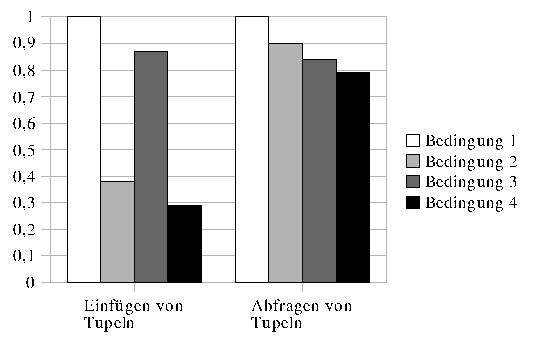
\includegraphics{fig/benchmark.pdf}
	\caption{Tolles Diagramm}
\label{fig:diagramm}
\end{figure}


\chapter{Zweites Inhaltskapitel}
	TODO


\chapter{Zusammenfassung}
	TODO Zusammenfassung



\backmatter
\bibliographystyle{alphadin}
\bibliography{bib/literatur}
%\nocite{*}

\end{document}
